
% III.D. Target-Domain Residual Pressure Prediction

\subsection{Target-Domain Residual Pressure Prediction}
\label{sec:target-residual}

The hierarchical pressure prior developed in Sec.~\ref{sec:knowledge-projection} captures the sectional aerodynamic response and the transferred finite-span corrections, but does not fully resolve the three-dimensional pressure variations of the target configuration. The remaining discrepancy is defined as
\begin{equation}
R_{p,s}^{\mathrm{tar}}(\eta,\xi)
=
C_{p,s}^{3D,\mathrm{CFD}}(\eta,\xi)
-
C_{p,s}^{\mathrm{prior}}(\eta,\xi),
\quad s\in\{u,l\},
\label{eq:target-residual-definition}
\end{equation}
where $\eta$ and $\xi$ denote the normalized spanwise and chordwise coordinates, respectively. Rather than reconstructing the entire pressure field from target-domain samples, the residual model learns the pressure variations not adequately represented by the transferred knowledge. At each forward pass, the pressure prior is recomputed using the current regional gating and amplitude parameters, ensuring consistency between the network input and the reconstructed pressure.

The target-domain network combines target-wing geometric and flow information, an explicit hierarchical pressure prior, and latent features extracted from the frozen sectional baseline model. The pressure prior provides an initial aerodynamic reference field incorporating the sectional baseline response and the transferred root- and tip-region corrections. It also serves as an explicit input to the residual network. The frozen L1 sectional features, extracted after global feature fusion in the sectional model, are introduced into the upper- and lower-surface streams through separate trainable adapters. Thus, the transferred knowledge contributes both an initial pressure estimate and a learned representation of sectional aerodynamic characteristics.

As illustrated in Fig.~\ref{fig:target-residual-architecture}, the residual network employs a partially shared dual-surface architecture. Separate local encoders first extract chordwise features from the upper and lower surfaces. The corresponding frozen sectional features are transformed through surface-specific trainable adapters and combined with the local representations. The resulting features are then processed by separate multiscale axial residual convolutional networks (ResCNNs) with surface-specific weights, followed by spanwise Transformers with shared weights. Although the Transformer parameters are shared, the upper- and lower-surface features are processed separately. At each fixed chordwise location, the Transformers capture interactions among spanwise sections, using the normalized spanwise coordinate, local-to-root chord ratio, and root- and tip-based integrated chord counts as positional features.

Cross-surface coupling is subsequently introduced through an additional global spanwise interaction branch. This branch first pools the features of each surface along the chordwise direction, jointly processes the combined spanwise representations, and redistributes the resulting contextual information to the corresponding surface streams. This operation enables information exchange between the upper and lower surfaces while retaining their separate local feature representations. Independent residual heads then predict the pressure corrections for the two surfaces.

\begin{figure*}[t]
    \centering
    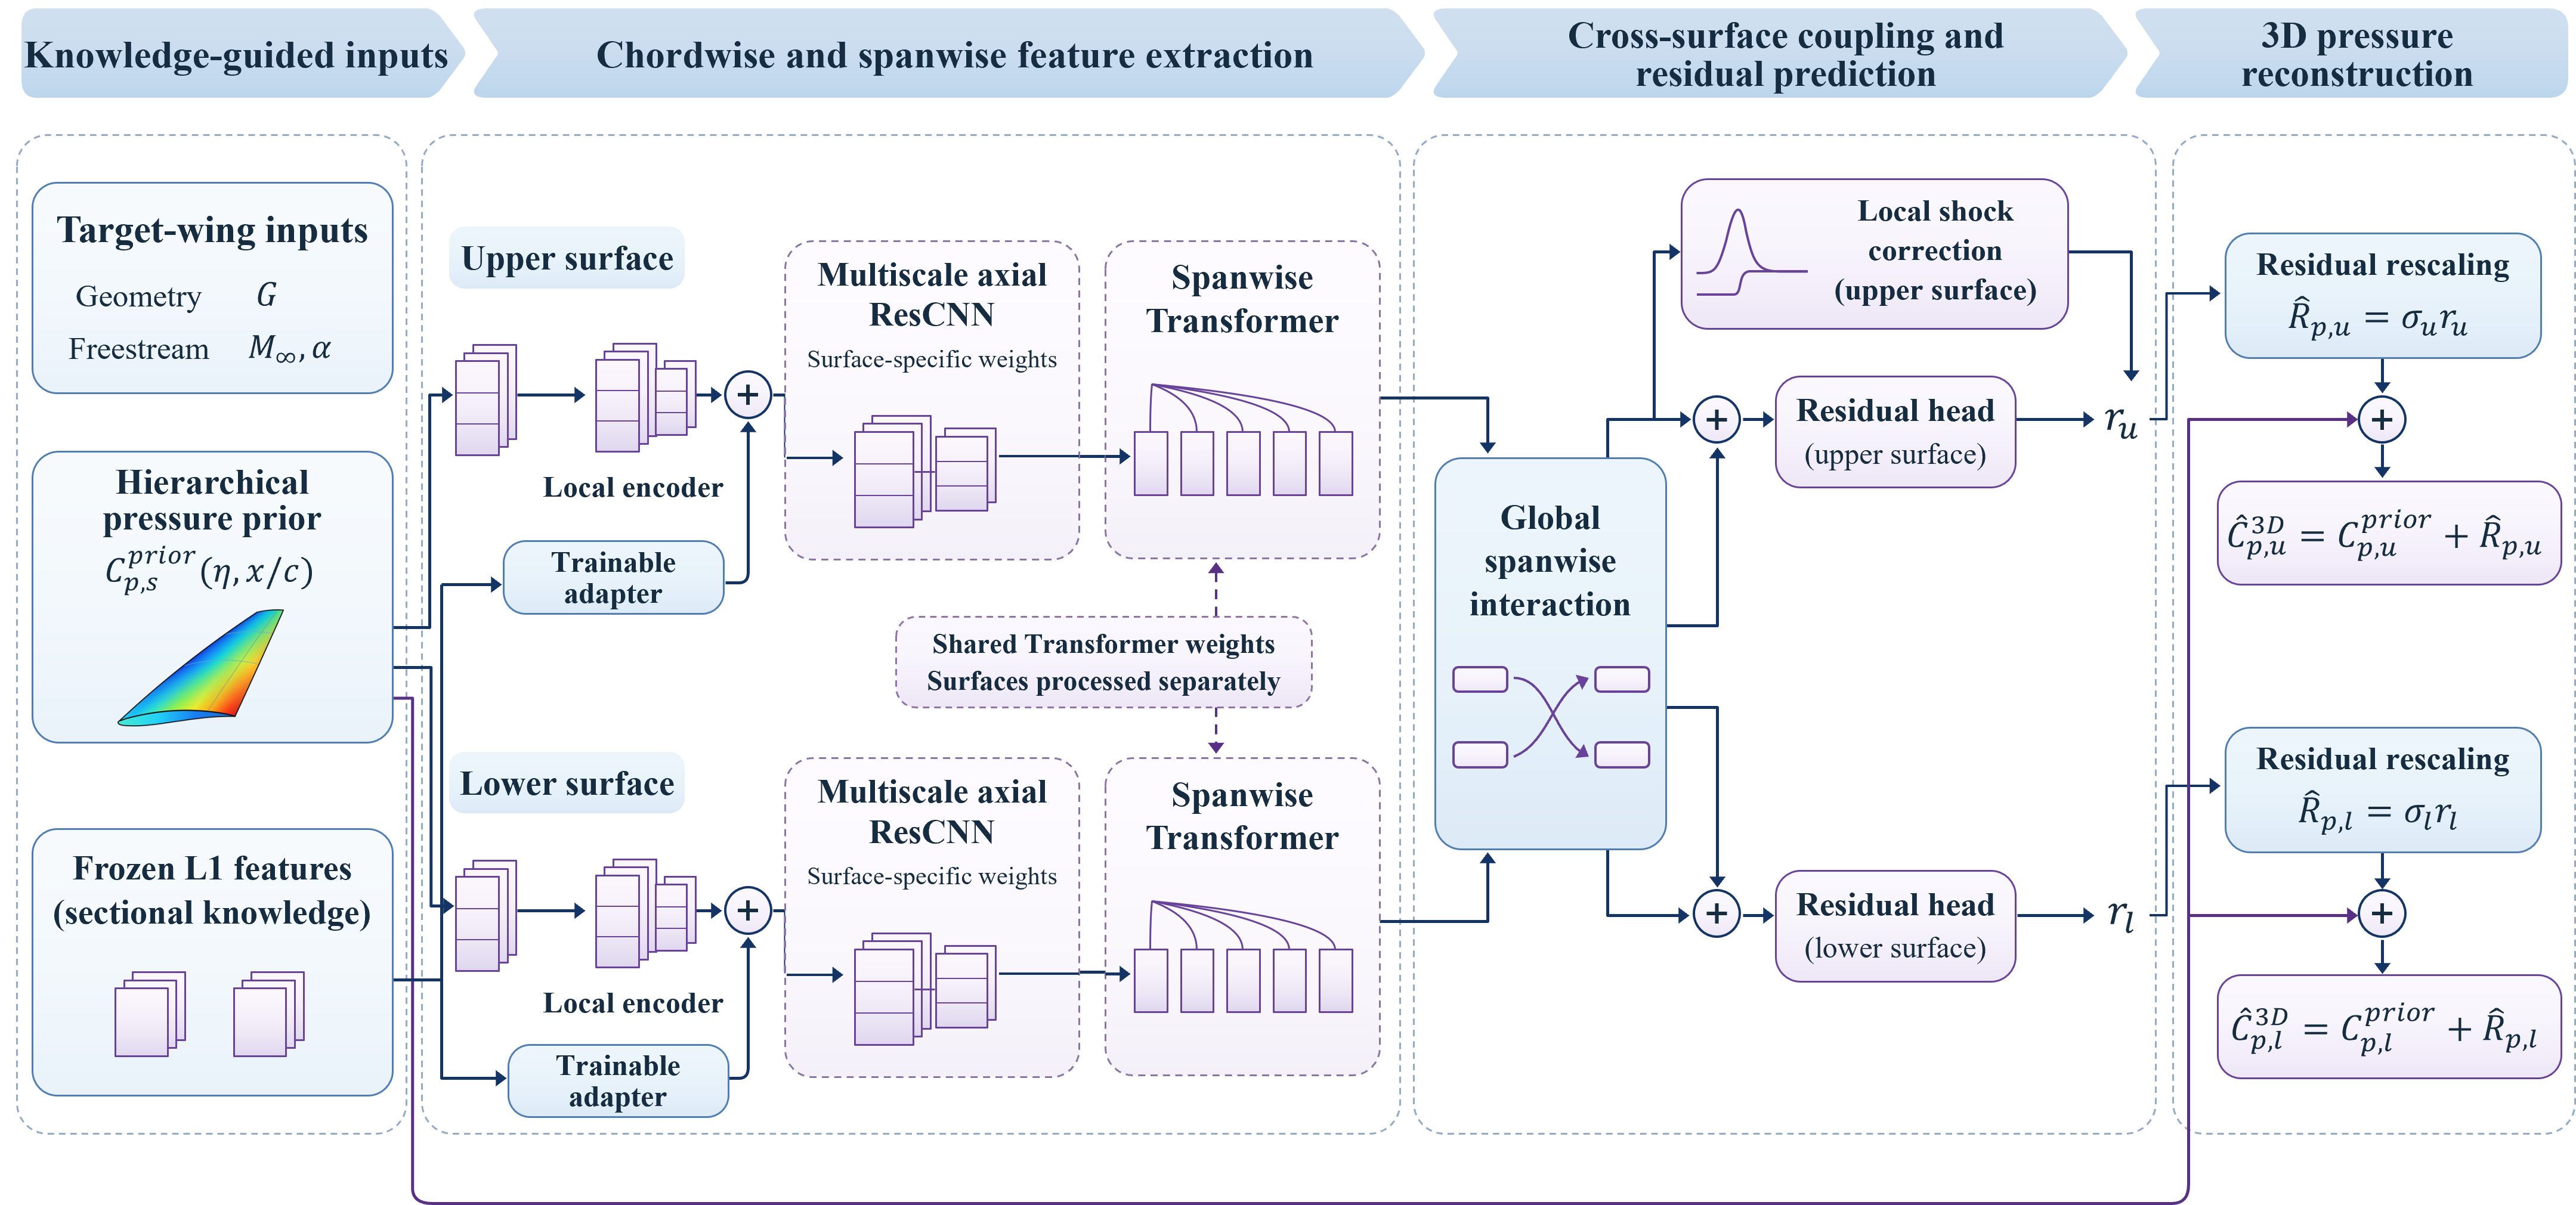
\includegraphics[width=0.98\textwidth]{III_Knowledge_Transfer/figures/III_D_Fig12/III_D_Fig12_target_residual_architecture.png}
    \caption{Architecture of the target-domain residual network}
    \label{fig:target-residual-architecture}
\end{figure*}

To provide an additional representation of abrupt pressure changes in transonic flow, a parametric shock-correction branch is applied to the upper surface. A reference location is estimated from the positive chordwise pressure gradient of the current pressure prior. Based on this reference, the network predicts a location shift, a characteristic width, a presence factor, and two correction amplitudes. The resulting parametric correction is added to the conventional upper-surface residual prediction, giving the standardized residual:
\begin{equation}
\begin{aligned}
r_u &= r_u^{\mathrm{head}}+p_{\mathrm{sh}}(A_G G+A_S S),\\
G &= \exp\left[-\frac{1}{2}\left(\frac{d}{w}\right)^2\right],\\
S &= \operatorname{sigmoid}\left(\frac{d}{w}\right).
\end{aligned}
\label{eq:upper-shock-correction}
\end{equation}

Here, $r_u^{\mathrm{head}}$ denotes the conventional upper-surface residual, and $d=\xi-\xi_{\mathrm{sh}}(\eta)$ is the distance from the predicted correction center. The parameters $w(\eta)$ and $p_{\mathrm{sh}}(\eta)$ represent the correction width and shock-presence factor, respectively, while $A_G(\eta)$ and $A_S(\eta)$ control the amplitudes of the Gaussian and sigmoid components. The dependence of $r_u$, $G$, and $S$ on $(\eta,\xi)$ is omitted for brevity. The correction center and presence logit receive explicit auxiliary supervision from target-domain CFD, whereas the width and amplitude parameters are learned through the reconstructed pressure.

The standardized residuals are converted into physical pressure-coefficient increments using surface-specific, zero-centered residual root-mean-square (RMS) scales computed from the target-domain training samples. The final prediction is
\begin{equation}
\widehat C_{p,s}^{3D}(\eta,\xi)
=
C_{p,s}^{\mathrm{prior}}(\eta,\xi)
+
\sigma_s r_s(\eta,\xi),
\quad s\in\{u,l\},
\label{eq:target-pressure-reconstruction}
\end{equation}
where $\sigma_s$ denotes the training-derived residual RMS scale for surface $s$. Zero initialization of the residual output heads and the shock-correction amplitude channels makes the initial prediction identical to the hierarchical pressure prior. The physical residual is subsequently learned without a final hyperbolic-tangent amplitude restriction.

The primary training objective is the pointwise mean squared error of the reconstructed pressure coefficients. Let $\mathcal V$ denote the set of valid surface nodes over the training batch, excluding the first chordwise node on each surface and the topologically degenerate exact tip section. The pressure loss is defined as
\begin{equation}
\mathcal L_{C_p}
=
\frac{1}{|\mathcal V|}
\sum_{(j,s,i)\in\mathcal V}
\left(
\widehat C_{p,s}^{3D,j}(\xi_i)
-
C_{p,s}^{3D,\mathrm{CFD},j}(\xi_i)
\right)^2,
\label{eq:target-pressure-mse}
\end{equation}
where $j$, $s$, and $i$ index the spanwise section, surface, and chordwise node, respectively. This normalization assigns equal weight to each valid pressure node, rather than assigning equal weight to the upper- and lower-surface mean squared errors.

Although the pointwise pressure loss constrains the reconstructed field, it does not explicitly distinguish the location, magnitude, or occurrence of localized pressure rises. Three auxiliary terms are therefore introduced for the upper surface. Reference features are derived from the positive chordwise pressure gradients of the CFD training labels at interval midpoints
\begin{equation*}
\bar{\xi}_i=\frac{\xi_i+\xi_{i+1}}{2},
\qquad 0.08\leq\bar{\xi}_i\leq0.85.
\end{equation*}
A section is considered to exhibit a pronounced pressure rise when its maximum positive gradient is at least 3.0. A softmax-weighted gradient centroid provides the reference location, while a similarly weighted sum of positive adjacent-node pressure increments characterizes the local pressure-rise magnitude. Both sets of gradient weights use the CFD reference peak, bounded below by 3.0, for normalization and a softmax temperature of 8.0. The latter descriptor is not a direct measure of the total shock pressure jump.

The location term applies a Smooth-$L_1$ penalty to the shock-correction center predicted by the network, using a chordwise normalization scale of 0.10. The magnitude term compares the pressure-rise descriptors evaluated from the final reconstructed and CFD pressure fields, normalized by the reference magnitude with a lower bound of 0.05. These two terms are computed only for sections with a detected pressure rise. In contrast, the presence term uses binary cross-entropy with logits for all valid sections, including those without a detected pressure rise. If no section is detected, the location and magnitude terms are set to zero.

The resulting training objective is
\begin{equation}
\begin{aligned}
\mathcal L={}&
\mathcal L_{C_p}
+\lambda_{\mathrm{pos}}\mathcal L_{\mathrm{pos}}\\
&+\lambda_{\mathrm{str}}\mathcal L_{\mathrm{str}}
+\lambda_{\mathrm{pres}}\mathcal L_{\mathrm{pres}},
\end{aligned}
\label{eq:target-total-loss}
\end{equation}
where $\mathcal L_{\mathrm{pos}}$, $\mathcal L_{\mathrm{str}}$, and $\mathcal L_{\mathrm{pres}}$ denote the location, pressure-rise magnitude, and presence losses, respectively. Their weights are fixed at
\begin{equation*}
\lambda_{\mathrm{pos}}=2\times10^{-4},
\qquad
\lambda_{\mathrm{str}}=10^{-4},
\qquad
\lambda_{\mathrm{pres}}=5\times10^{-5}
\end{equation*}
throughout training. The reference features and presence labels are computed from CFD data for training only; no reference pressure or CFD-based detection is required at inference.
